\chapter{Empirical Evaluation}\label{experiments}
In this chapter we are going to focus on the analysis of the different experiments that we have conducted
to respond our research questions that emerged from the motivation of this work. 

\section{Research Questions}
The fundamental part of this work is focus on incremental enumeration. Although this there are other areas that 
it is important to explore beyond that: memory consumption, thread scheduling, execution time and query comparison.

In that sense we have asked the following research question that we try to answer with the conducted experiments:
\begin{inparaenum}[\bf {\bf RQ}1\upshape)]
\label{res:bt:question}
    \item Does \acrshort{dpbt} generates incremental results regardless the size of the graph?
    \item Does the type of query $Q$ impacts on either the execution of \acrshort{dpbt}?
    \item Does \acrshort{dpbt} follows a \emph{pay-as-you-go} model?
    \item Does \acrshort{dpbt} handle memory and threads efficiently?
\end{inparaenum}
  
\section{Experiments}

We have conducted different kinds of experiments to test our assumptions and verify the correctness of the implementation.
First, we have performed a \emph{Diefficiency Metrics Analysis}~\cite{diefpaper} in order to asses the incremental capabilities of the solution. 
Then we have performed a \emph{Benchmark Analysis} to identify how the algorithm varies depending of the type of query command selected for the user.
Finally, we have executed a \textit{Performance Analysis} in which we have to gather profiling data from \acrfull{ghc} for one of the graphs, 
to measure how the program performs regarding multithreading and memory allocation.

\subsection{Running Architecture}
All the experiments have been executed in a $x86$ $64$ bits architecture with a \textit{$6$-Core Intel Core i7} processor of $2,2$ GHz which can emulate up to $12$ virtual cores. 
This processor has \emph{hyper-threading} enable. Regarding memory, the machine has $32 GB$ \emph{DDR4} of RAM, $256\ KB$ of L2 cache memory, and $9\ MB$ of L3 cache.

\subsection{Haskell Setup}
Regarding specific libraries and compilations flags used on \acrshort{hs}, we have used \acrshort{ghc} version $8.10.4$. We have also used the following set of libraries: 
\mintinline{bash}{dyanmic-pipeline 0.3.2.0} \cite{dynamic-pipeline}, \mintinline{bash}{bytestring 0.10.12.0} \cite{bytestring}, \mintinline{bash}{containers 0.6.2.1} \cite{containers}, 
\mintinline{bash}{relude 1.0.0.1} \cite{relude} and \mintinline{bash}{unagi-chan 0.4.1.3} \cite{unagi}. The use of \texttt{relude} library is because we disabled 
\mintinline{haskell}{Prelude} from the project with the language extension \mintinline{haskell}{NoImplicitPrelude} \cite{extensions}. Regarding compilation flags 
(\acrshort{ghc} options) we have compiled our program with \mintinline{bash}{-threaded}, \mintinline{bash}{-O3}, \mintinline{bash}{-rtsopts}, \mintinline{bash}{-with-rtsopts=-N}. 
Since we have used \texttt{stack} version $2.5.1$ \cite{stack} as a building tool on top of \acrshort{ghc} the compilation command is \mintinline{bash}{stack build}\footnote{For more information about package.yaml or cabal file please check https://github.com/jproyo/upc-miri-tfm/tree/main/bt-graph-dp}.

\subsection{DataSets}\label{data:set}

For all the experiments, we have used the following networks taken from Konect Networks~\cite{konect}. In this particular experiment setup, we have selected the following specific data sets that can be found here \cite{konect:2017:dbpedia-recordlabel,konect:2017:moreno_crime,konect:2017:opsahl-ucforum,konect:2017:wang-amazon}

\begin{table}[H]
  \centering
  \begin{tabular}{|p{0.25\linewidth}|c|c|c|c|c|}
    \hline
   \textbf{Network} & \textbf{$|U|$} & \textbf{$|L|$} & \textbf{$|E|$} & \textbf{Wedges} & \textbf{\#\acrshort{bt}} \\
   \hline
   Dbpedia & 18422 & 168338 & 233286 & $1.45 \times 10^8$ & $3.62 \times 10^8$\\
   \hline
   Moreno Crime & 829 & 551 & 1476 & 4816 & 211\\
   \hline
   Opsahl UC Forum  & 899 & 522 & 33720 & 174069 & $2.2 \times 10^7$ \\
   \hline
   Wang Amazon & 26112 & 799 & 29062 & $3.4 \times 10^6$ & 110269\\
   \hline
  \end{tabular}
 \caption{DataSet of selected \acrlong{bg}}
 \label{table:exp:data-set}
 \end{table}
 
The criteria for selecting those networks has followed the idea of first do the analysis over at least one for the big networks~\cite{konect:2017:dbpedia-recordlabel} used on the \acrshort{bt} counting work~\cite{btcount}.
Then we selected some networks more from the same data source~\cite{konect} with different size and topology.

\subsection{Experiments Definition}\label{sub:exp:exp-def}
\paragraph{E1: Diefficiency Metrics Analysis}\label{sub:sec:exp-1} In this experiment we asses the ability of \acrshort{dpbt} to generate results incrementally.
In order to do that, we use \acrfull{dm} Tool \emph{diefpy}~\cite{diefpy} which implements \emph{Diefficiency Metrics} explain in his work~\cite{diefpaper}.
Conducting this experiment allow us to answer research question [R1] and [R3] defined in \autoref{res:bt:question}. 

\paragraph{E2: Benchmark Analysis}\label{sub:sec:exp-2} In this case we want to answer research question [R2] in order to know what is the impact of enumerating some \acrshort{bt} that follow certain criteria. 
This also will indirectly answer [R3] because if we see a difference of the results based on the type of the command we are going to be able to answer that question. This is done over the same data set and 
experiment setup used previously in \autoref{sub:sec:exp-1}, but without \emph{\acrshort{dbpedia}} network and using \mintinline{shell}{criterion} \cite{criterion} benchmark tool.

\paragraph{E3: Performance Analysis}\label{sub:sec:exp-3} Finally we will take measurements on one network only about the use of memory and threads on \acrshort{ghc}, using
\mintinline{shell}{ThreadScope} \cite{threadscope} and \mintinline{shell}{eventlog2html} \cite{eventlog2html} tools. 

\subsection{Experiments Data Setup}\label{sub:exp:exp-data-setup}
For the case of \autoref{sub:sec:exp-1} and \autoref{sub:sec:exp-2} we defined the following scenarios to conduct all the experiments regardless the network used.
In the case of the \emph{Description} column \emph{"Seach"} stands for \emph{"Seach all Bi-triangles that matches with.."}.
A \emph{low, high and medium incidence level} means the following:
\begin{inparaenum}
  \item[Low] A vertex or edge that is appearing in less than $5\%$ of the total number of edges
  \item[Medium] A vertex or edge that is appearing between $5\%-25\%$ of the total number of edges
  \item[Low] A vertex or edge that is appearing in more than $25\%$ of the total number of edges
\end{inparaenum}
The selection criteria is random on all cases and for detecting the incidence level we have analyze the source Data
and check how the vertex or edge is connected with the rest of graph.

\begin{table}[H]
  \centering
  \begin{tabular}{|l|c|c|}
    \hline
   \textbf{Setup ID} & \textbf{Name} & \textbf{Search by}\\
   \hline
   E-H & Edge High & edge with high incidence \\
   \hline
   E-L & Edge Low & edge with low incidence \\
   \hline
   E-M & Edge Medium & edge with medium incidence \\
   \hline
   VL-H & $l \in L$ High & vertex in lower layer with high incidence \\
   \hline
   VL-L & $l \in L$ Low & vertex in lower layer with low incidence \\
   \hline
   VL-M & $l \in L$ Medium & vertex in lower layer with medium incidence \\
   \hline
   VU-H & $u \in U$ High & vertex in upper layer with high incidence \\
   \hline
   VU-L & $u \in U$ Low & vertex in upper layer with low incidence \\
   \hline
   VU-M & $u \in U$ Medium & vertex in upper layer with medium incidence \\
   \hline
  \end{tabular}
 \caption{Experiment Data Setup for experiments}
 \label{table:exp:data-setup}
 \end{table}

\section{\textbf{Discussion over Observed Results}}\label{sec:discussion}
\subsection{Experiment: E1}\label{sub:sec:res:e1}
Regarding the results obtained by \acrshort{dm} tool, the data is presented in two different formats by it: the graphics that show 
how the different results are enumerated in each point of the time, and a radial graphic that shows the tension between aspects of the time measurement.
One important thing to point out about this graphs and data is that the time represents the amount of nanoseconds elapsed to deliver that result from the moment 
the \acrshort{dpbt} finishes the execution of $\ac$ and it is executing $\ad$, therefore it is able to start processing commands. Then time $0$ is equal to start 
of $\ad$ execution.

\begin{figure}[!htb]
  \centering
  \begin{minipage}{0.5\textwidth}
   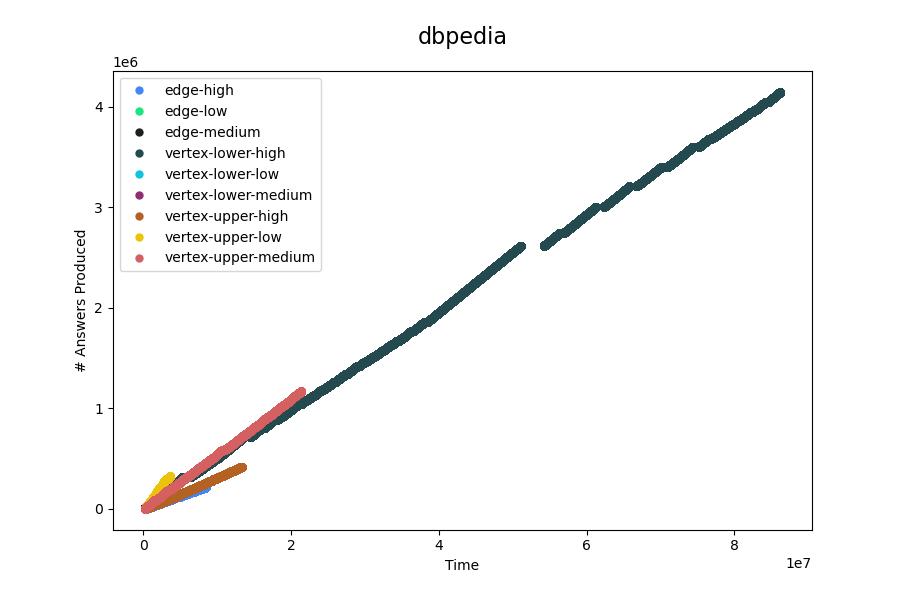
\includegraphics[width=1\linewidth, height=0.2\textheight]{experiments/diepfy/dbpedia.png}
    \caption{\acrshort{dbpedia} \acrshort{dm}}
    \label{fig:dief:dbpedia}
  \end{minipage}%
  \begin{minipage}{0.5\textwidth}
   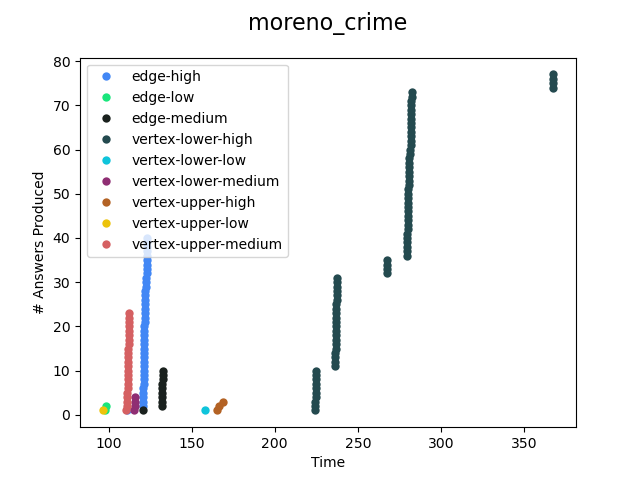
\includegraphics[width=1\linewidth, height=0.2\textheight]{experiments/diepfy/moreno_crime.png}
    \caption{Moreno Crime \acrshort{dm}}
    \label{fig:dief:moreno}
  \end{minipage}
\end{figure}
%
\begin{figure}[!htb]
  \centering
  \begin{minipage}{0.5\textwidth}
   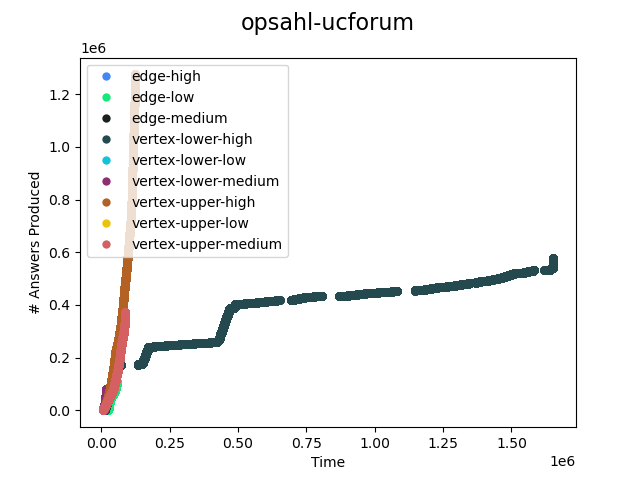
\includegraphics[width=1\linewidth, height=0.2\textheight]{experiments/diepfy/opsahl-ucforum.png}
    \caption{Opsahl UC Forum \acrshort{dm}}
    \label{fig:dief:opsahl}
  \end{minipage}%
  \begin{minipage}{0.5\textwidth}
    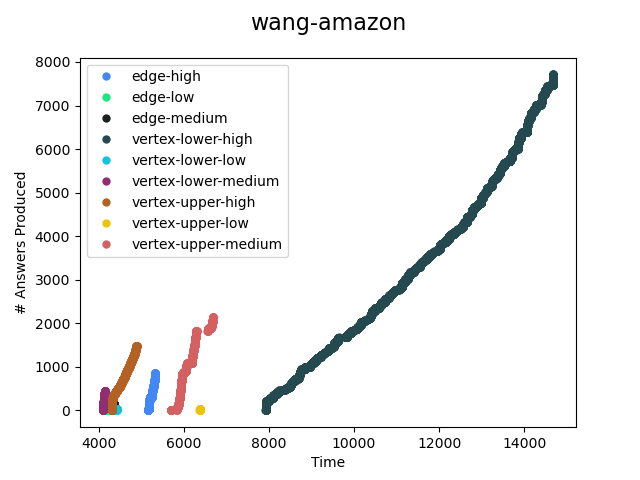
\includegraphics[width=1\linewidth, height=0.2\textheight]{experiments/diepfy/wang-amazon.png}
     \caption{Wang Amazon \acrshort{dm}}
     \label{fig:dief:wang}
   \end{minipage}
 \end{figure}

As we can appreciate in the results above for all the data sets and for each of the experiments \acrshort{bt} are incrementally 
enumerated and deliver to the user. In all the cases above, we seen how the experiment VL-H (see \autoref{table:exp:data-setup}), 
is the one with more incremental deliver of results to the user because it progressively delivering the results from some point in 
time until the end and not everything in one point. This case can be seen clearly because since we are aggregating bi-triangles based on 
some triple $(l_l,l_m,l_u)$ (see \dref{def:abt}), if the requested $l \in L$ matches with some of these triple elements, 
we need to enumerate all the $\ati$ there and since this is experiment is for $l$ with High incidence, there are many of them in the set.
Therefore we are going to deliver several of them progressively.
The only case that is not following this pattern is \autoref{fig:dief:opsahl}. That is explained because it is an outlier for this experiments.
Since the selection is random, it seems that for this particular experiment the selected vertex is not participating in many \acrshort{bt} as it should.
In fact it can be seen that for VU-H, the selection was good but the speed of the deliver didn't allow to see the incremental part\footnote{Check that the y-axis in the case of opsahl-ucforum and \acrshort{dbpedia} is $10^6$ scale as it is indicated on top of the graphic}. 
The case of Moreno Crime in \autoref{fig:dief:moreno} that seems the least incremental one, it is explain by the fact of the topology of the graph, which is the smallest one 
in terms of number of \acrshort{bt} and number of wedges. Therefore it is extremely fast how the results are generated and incremental results only can be appreciated in the vertices with high incidence.

\begin{figure}[!htb]
  \centering
  \begin{minipage}{0.5\textwidth}
   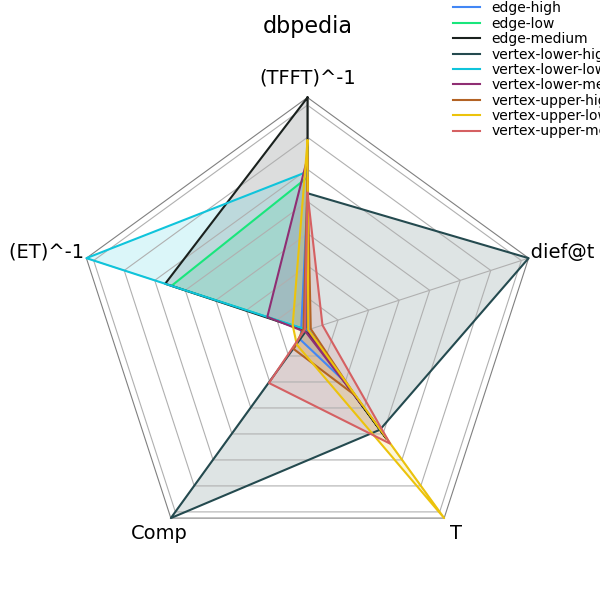
\includegraphics[width=1\linewidth, height=0.3\textheight]{experiments/diepfy/dbpedia_radial.png}
    \caption{\acrshort{dbpedia} \acrshort{dm} - Radial}
    \label{fig:dief:dbpedia-radial}
  \end{minipage}%
  \begin{minipage}{0.5\textwidth}
   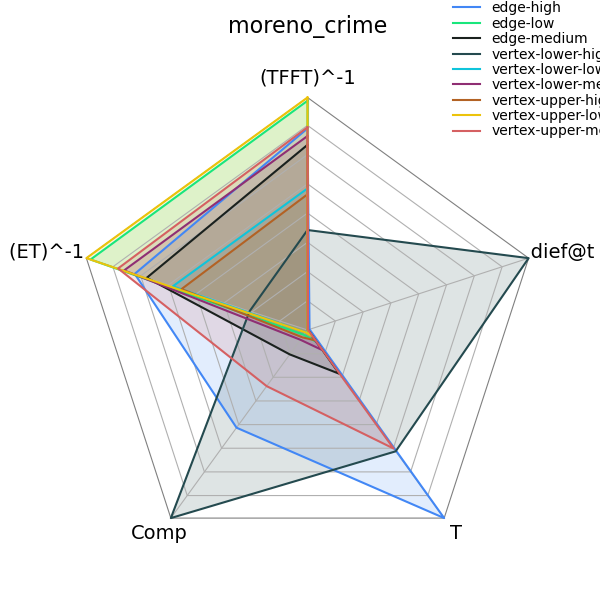
\includegraphics[width=1\linewidth, height=0.3\textheight]{experiments/diepfy/moreno_crime_radial.png}
    \caption{Moreno Crime \acrshort{dm} - Radial}
    \label{fig:dief:moreno-radial}
  \end{minipage}
\end{figure}
%
\begin{figure}[!htb]
  \centering
  \begin{minipage}{0.5\textwidth}
   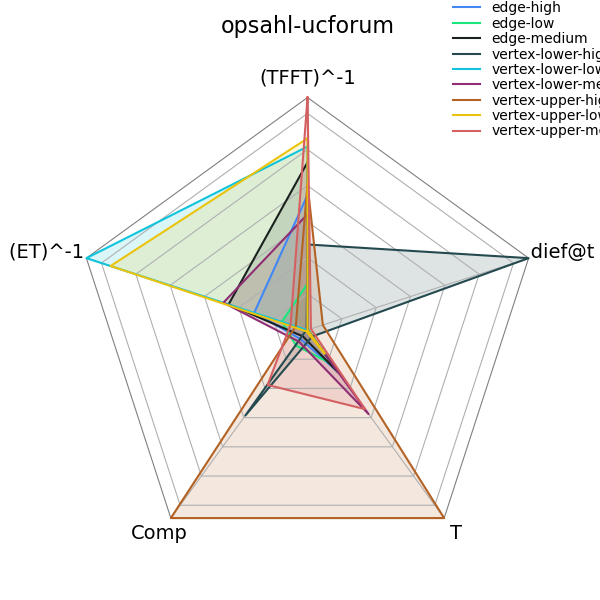
\includegraphics[width=1\linewidth, height=0.3\textheight]{experiments/diepfy/opsahl-ucforum_radial.png}
    \caption{Opsahl UC Forum \acrshort{dm} - Radial}
    \label{fig:dief:opsahl-radial}
  \end{minipage}%
  \begin{minipage}{0.5\textwidth}
    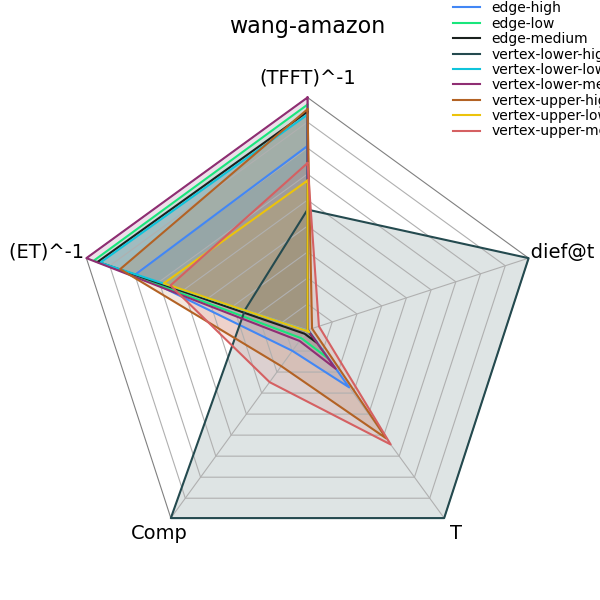
\includegraphics[width=1\linewidth, height=0.3\textheight]{experiments/diepfy/wang-amazon_radial.png}
     \caption{Wang Amazon \acrshort{dm} - Radial}
     \label{fig:dief:wang-radial}
   \end{minipage}
 \end{figure}

These radial plots obtained from \acrshort{dm} shows the tension between \acrfull{dt} (higher better),
\acrfull{et}, \acrfull{tfft}, \acrfull{comp} and finally \acrfull{tt}. A perfect cover of all the radial area with all the dimensions would
indicate a perfect solution with incremental delivery of results, completeness, throughput, etc. The important part to remark here which verify
our deduction from the other graphics is that all the VL-H tension over \acrshort{dt} metric indicating that they are incremental on that part. 
The rest of the data setup experiments indicates that the level of throughput, completeness and execution time is less and the results can be deliver
faster outlying incremental behavior. We know from the other graphics that is not true since there are more data setups which also deliver incremental 
results throughout time.

\paragraph{Conclusion E1} In conclusion we are able to answer [R1] and asses that we have built an incremental algorithm for enumerate \acrlong{bt}. 
The same conclusion can be obtained regarding question [R3] and verify that this is a \emph{pay-as-you-go} model, since depending on the requirement of the user, 
in this case the command and the query selected, the cost of obtaining faster or later the results but in an incremental manner are done.

\subsection{Experiment: E2}\label{sub:sec:res:e2}
As we can see in the definition of \mintinline{shell}{criterion} tool \cite{criterion}, the benchmark is conducting running the same experiments many times (by default 100 each),
to do an statistical analysis on the execution time, eliminating outliers and fitting a regression model that could explain that behavior. 
In this experiments we have conducted the benchmark using all the networks but not \acrshort{dbpedia} because of its size, and all the data setup described in \autoref{data:set}.

\begin{figure}[!htb]
  \begin{center}
     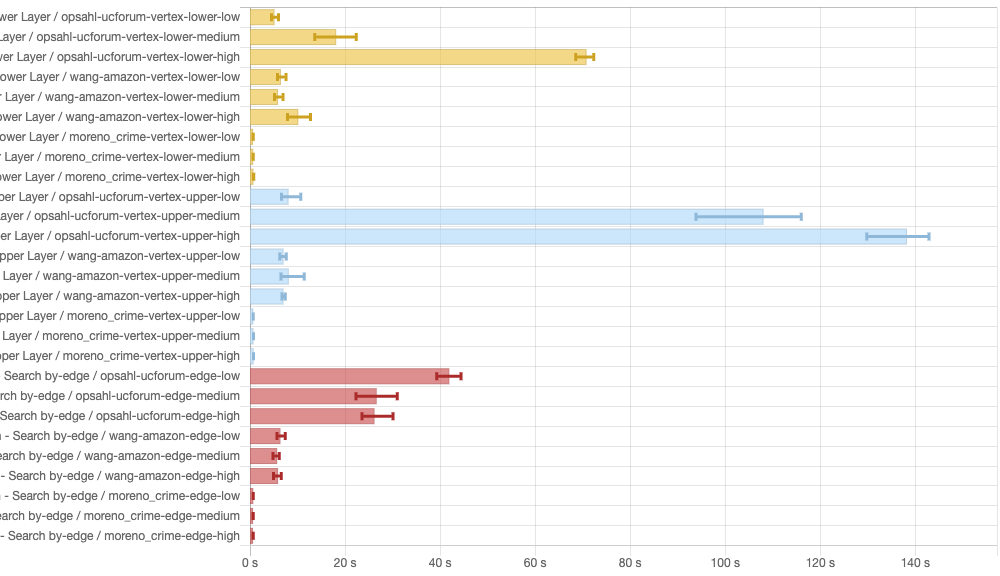
\includegraphics[width=1\textwidth] {experiments/bench_1}
       \end{center}
     \caption{Benchmark analysis}
     \label{fig:exp:bench}
 \end{figure}

As it can be seen in \autoref{fig:exp:bench}, yellow bars are all the experiments related to Lower Layer vertices, blue bar are related Upper Layer and 
red are the experiments related edges search. The most long bars which are taken more time are from opsahl-ucforum that we already know by \autoref{table:exp:data-set}, 
it is the biggest of three in terms of number of \acrshort{bt} and wedges, therefore it needs to enumerate more \acrshort{bt}. On the other hand almost all the high incidence
vertices and edges queries are taken longer as well. There is only one outlier which is E-H for opsahl-ucforum which could be explained by the randomize selection of it.

As we have explained, the tool fits a linear regression model with the observed empirical execution time.
We are leaving the details of all the data which is big in \autoref{app:exp:bench}.
From this data we can see that there is only one case where the model could not fit the data which is VU-L for opsahl-ucforum with an $R^2$ of $0.718$.
This could be explained by the fact of the variance in the samples which were a lower bound of $600$ms, estimate of	$2.43$s	and an upper bound of $3.18$s. 
This means that for some reason this experiment was not stable or predictable from the execution time point of view.

Another benchmark was not done with \mintinline{shell}{criterion} but was measure from \acrshort{dm} experiments the execution time of each experiment to compare them.

\begin{figure}[!htb]
  \begin{center}
     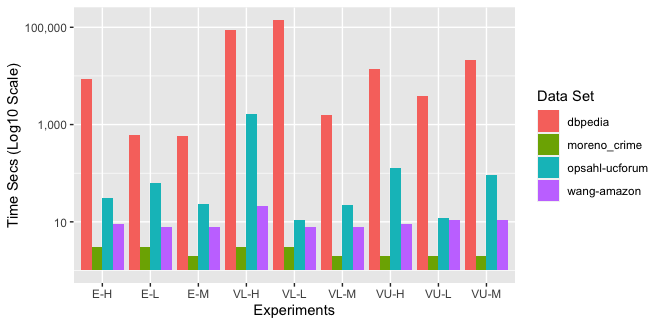
\includegraphics[width=1\textwidth] {experiments/execution_time_by_experiments}
       \end{center}
     \caption{Execution time comparison of all experiments}
     \label{fig:exp:bench:2}
 \end{figure}

\paragraph{Conclusion E2} We can answer the question [R2] because it can clearly be seen in the benchmark analysis and in \autoref{fig:exp:bench:2} that as long as the user request for more complex queries that involves more \acrshort{bt},
the execution time increases, therefore we are in a \emph{pay-as-you-go} model.

\subsection{Experiment: E3}\label{sub:sec:res:e3}
In these section we can divide the analysis in two: memory consumption and multi-threading.

\paragraph{Multithreading} Regarding multithreading we have gather different moments of Moreno Crime network run.\footnote{We could not conduct the analysis on bigger network due to the huge amount of data gather that make the program timeout running out of memory}.
As we can see in the overview execution in \autoref{fig:exp:perf:1} all the cores of this execution (8) are running 
threads and MUT time almost during all the execution of the program.
\begin{wrapfigure}{r}{0.5\textwidth}
  \begin{center}
     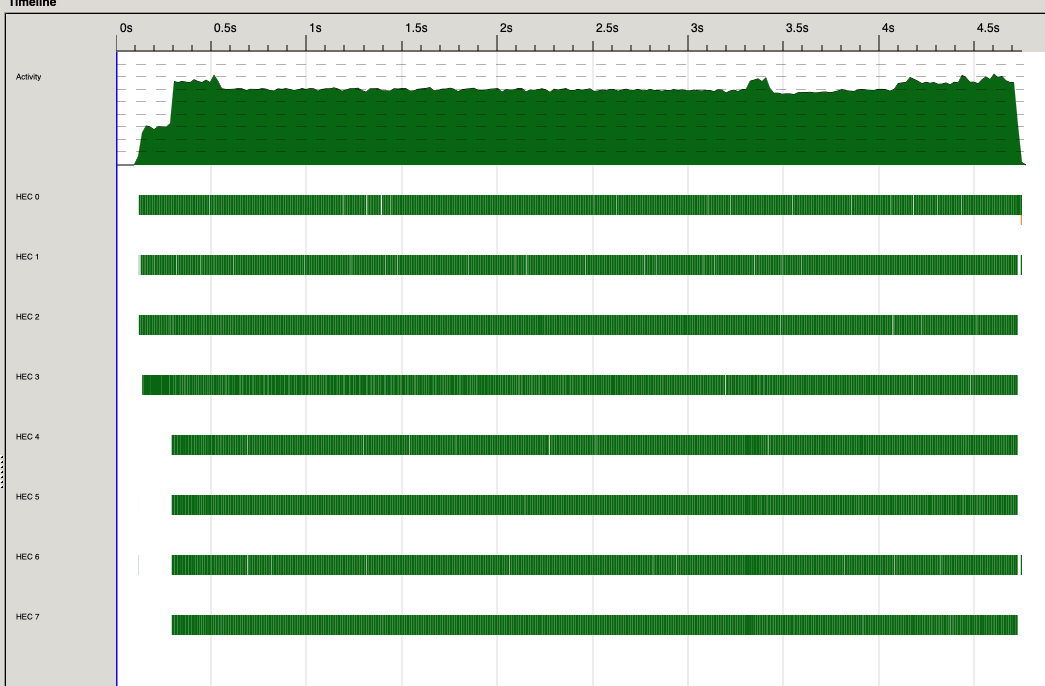
\includegraphics[width=0.48\textwidth] {experiments/thread/general_overview}
       \end{center}
     \caption{Threadscope - General overview}
     \label{fig:exp:perf:1}
 \end{wrapfigure}
That is a remarkable indicator in general indicating that GC pauses and running time is overtake by program and not GC. In fact \acrshort{ghc} productivity on this run indicated $99.8\%$.
If we zoom in at the beginning and at the end we are going to see that there is a moment when only 1 core it is executing. That fits perfect with the model since at the beginning \acrshort{dp}
setups all the filters and start reading the input file which is a single thread. Remember that each stage runs on its own thread. At the end also it is explained by the \acrshort{dp} paradigm 
because it happens the same but in the $\obt$.
In the middle of the execution where there is more processing of the $\fbt$, we can see that the threads are distributed evenly between the cores and the same 
behavior appears regarding less use of GC and higher MUT time.

\begin{figure}[!htb]
  \centering
  \begin{minipage}{0.3\textwidth}
   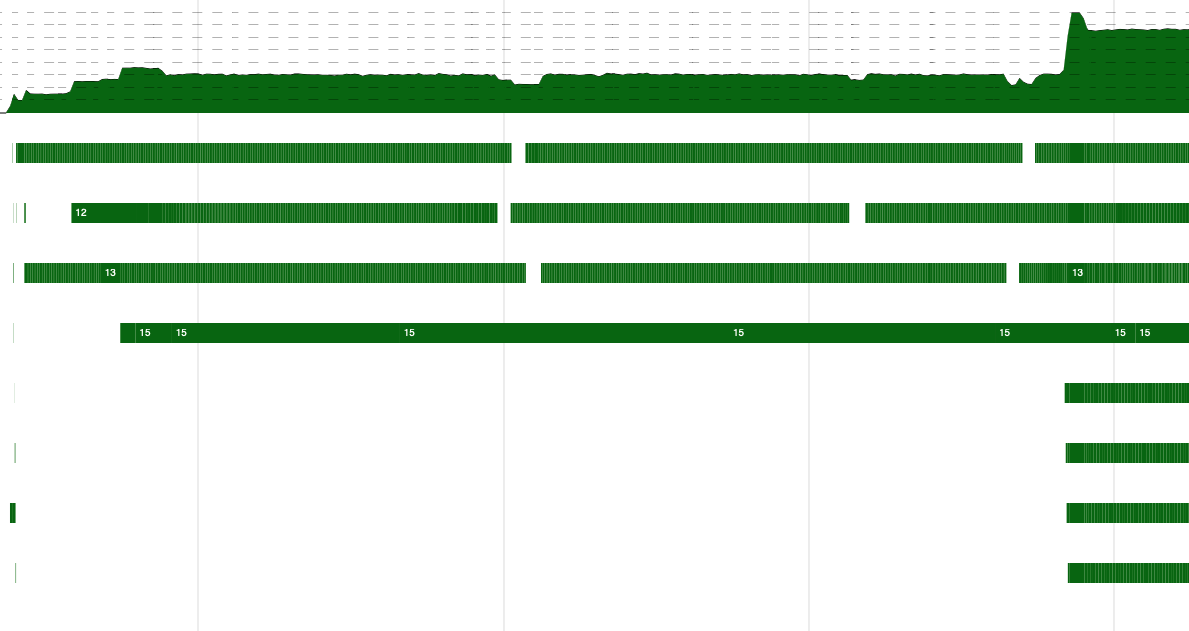
\includegraphics[width=1\linewidth, height=0.2\textheight]{experiments/thread/init}
   \caption{Init execution time}
   \label{fig:exp:perf:2}
  \end{minipage}%
  \hspace{.3cm}%
  \begin{minipage}{0.3\textwidth}
    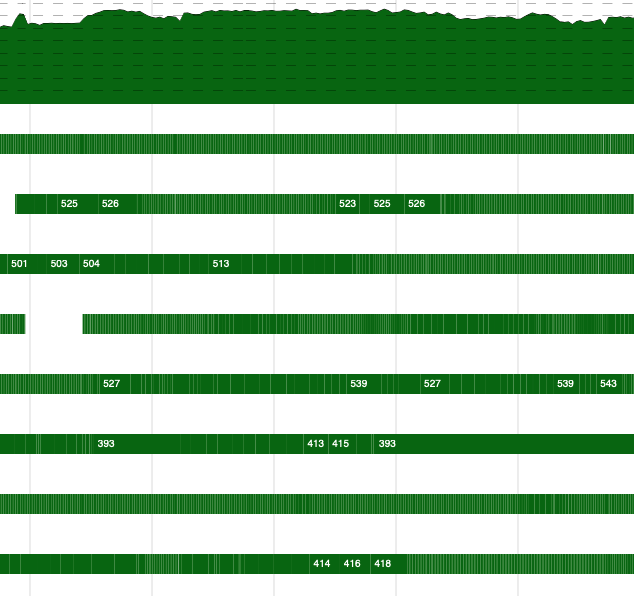
\includegraphics[width=1\linewidth, height=0.2\textheight]{experiments/thread/middle}
    \caption{Middle Execution time}
    \label{fig:exp:perf:4}
   \end{minipage}% 
   \hspace{.3cm}%
  \begin{minipage}{0.3\textwidth}
   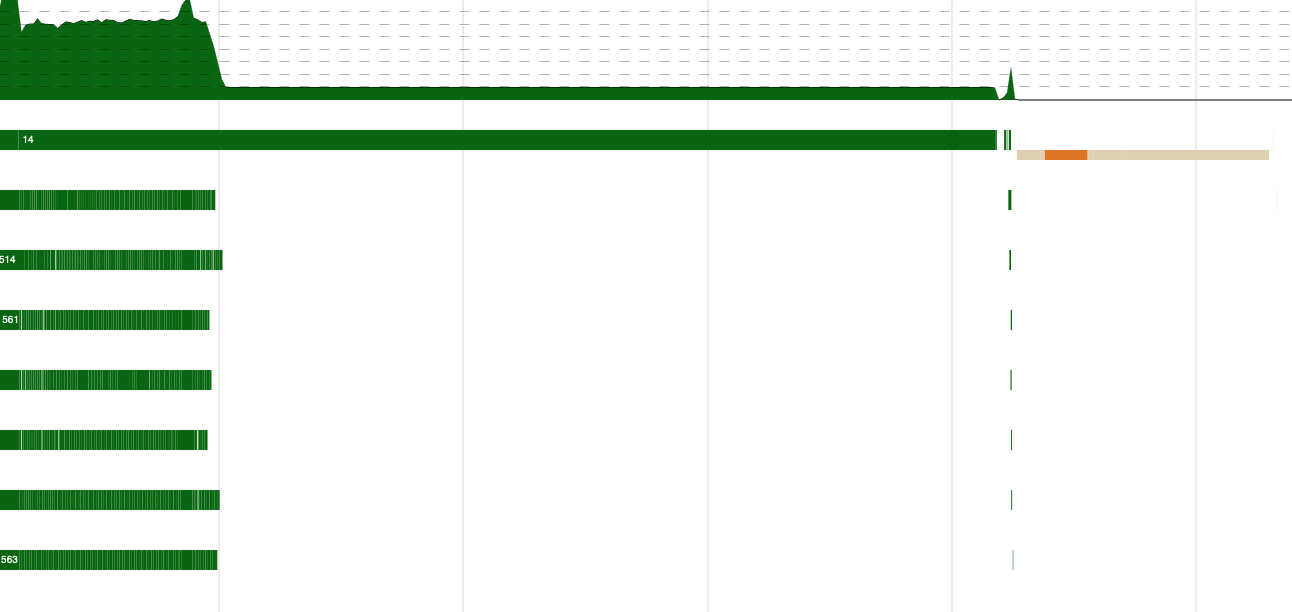
\includegraphics[width=1\linewidth, height=0.2\textheight]{experiments/thread/end}
   \caption{End execution time}
   \label{fig:exp:perf:3}
  \end{minipage}%
\end{figure}

\paragraph{Memory Consumption} In the case of memory consumption we have been able to measure
the memory consumption for the biggest graph which is \acrshort{dbpedia}. As it is known enabling profiling 
execution downgrade performance of execution time, and the execution for this case run out of memory
as we are going to see in the image, but we can gather interesting data to analyze memory allocation.

\begin{figure}[!htb]
  \begin{center}
     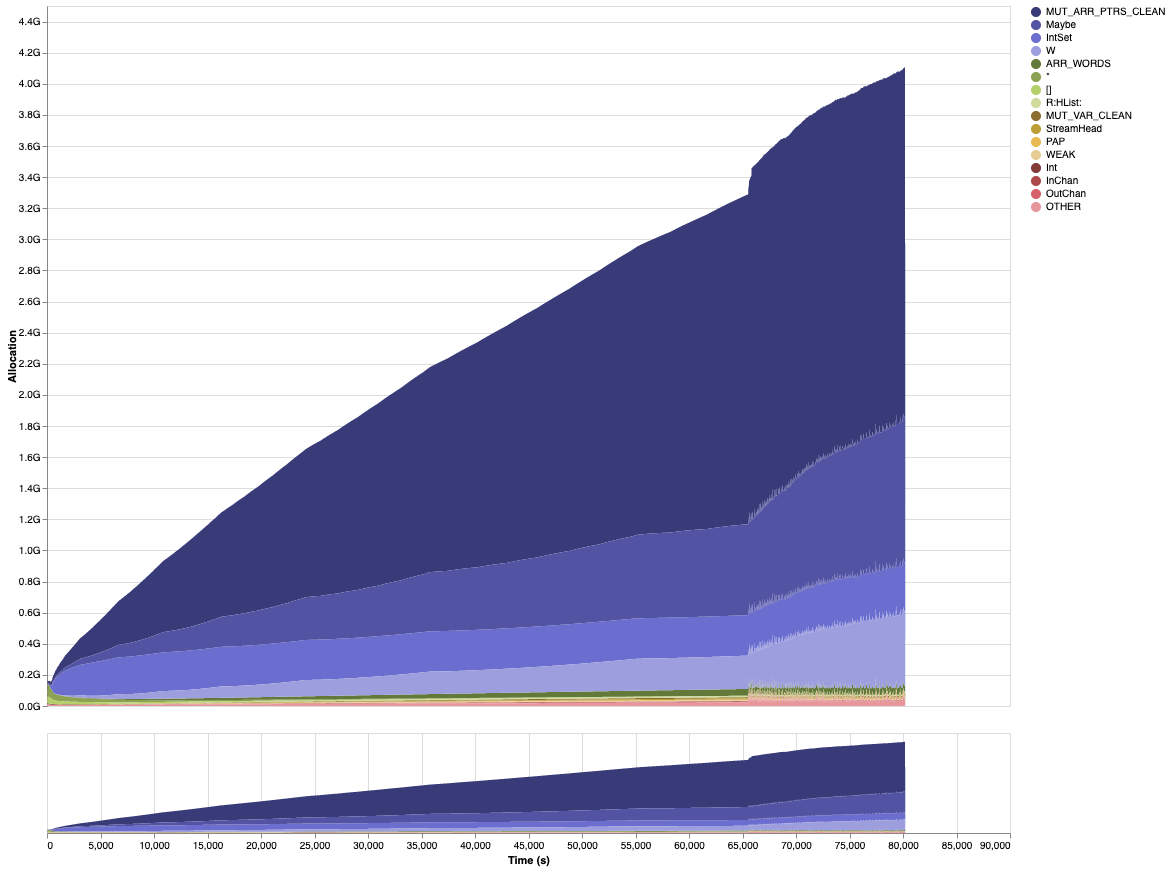
\includegraphics[width=1\textwidth] {experiments/mem/overview}
       \end{center}
     \caption{Memory allocation throughout execution time}
     \label{fig:exp:mem:1}
 \end{figure}

As we can appreciate in \autoref{fig:exp:mem:1} the darkest blue space belongs to \mintinline{shell}{MUT_ARR_PTRS_CLEAN}.
This type of objects are pointers to function. In \acrlong{hs} \mintinline{shell}{MUT} (mutator) is the acronym a thread evaluating a \acrshort{hs} expression.
That means that there are many pointers allocated waiting for evaluate expressions. This is perfectly explain by \acrshort{dp} model, in which we are spawning one
thread per stage, and in particular in \acrshort{dp} that means one thread per filter instance as well. In this case of \acrshort{dbpedia} which contains $168338$ vertices in 
$L$ according to \autoref{table:exp:data-set}, that means the same amount of thread for every run of this network. Since the execution of all this stage will not be 
released until it executes and finishes last $\ad$ (processing queries), all of them are waiting for the queries to be processed and executed.
The rest of the memory that is data flowing like \mintinline{haskell}{Maybe} and state of the filters instance \mintinline{haskell}{IntSet}, are less than $30\%$ of the 
total allocated memory as we can see. The linear fast growing of the memory could be explained for the reason exposed before. All the $\fbt$ instances are created as long
the program executes.

One of the tentative solution as a future work is to reduce the number of $\fbt$ for big graphs in order to reduce the number 
of allocated pointers.

\paragraph{Conclusion E3} We can answer question [R4] saying that we have shown that threads are efficiently handle by \acrshort{hs} \acrshort{ghc} scheduler supporting the 
parallelization level that \acrshort{dp} requires. On the other hand for completely answering the research question regarding memory consumption, although there is a penalty 
because of the size of the graph and the complexity of the problem, we believe that this aspect can be improved reducing the number of $\fbt$ instances and improving the data structures
used for searching and deliver \acrshort{bt}. It was out of the scope of this work to solve the efficiency of the queries and the underlying data structures involve to improve the efficiency. 

\section{Chapter Summary}
In this chapter we have explained in extended detail all the experiments conducted in order to answer our research question exposed.
We first started doing a summary of that research questions and after that we present the setup of the experiments, data and execution environment detail.
Then we describe the experiments and its results and we discussed about them deeply. At the end of each discussion experiment section we gave
a brief conclusion about the viability of answering the research questions.
